\chapter{提案手法}
\label{chap:propose}

\section{公開鍵暗号暗号方式による SSH を用いた登録・認証}
    \subsection{登録}
        ここでは,ここでは公開鍵暗号暗号方式による SSH を用いた認証から,WEBサービスの認証につなげる実装について記述する.
        以下の図\ref{registration}は実証の処理を記述した図である.
        \begin{figure}[H]
            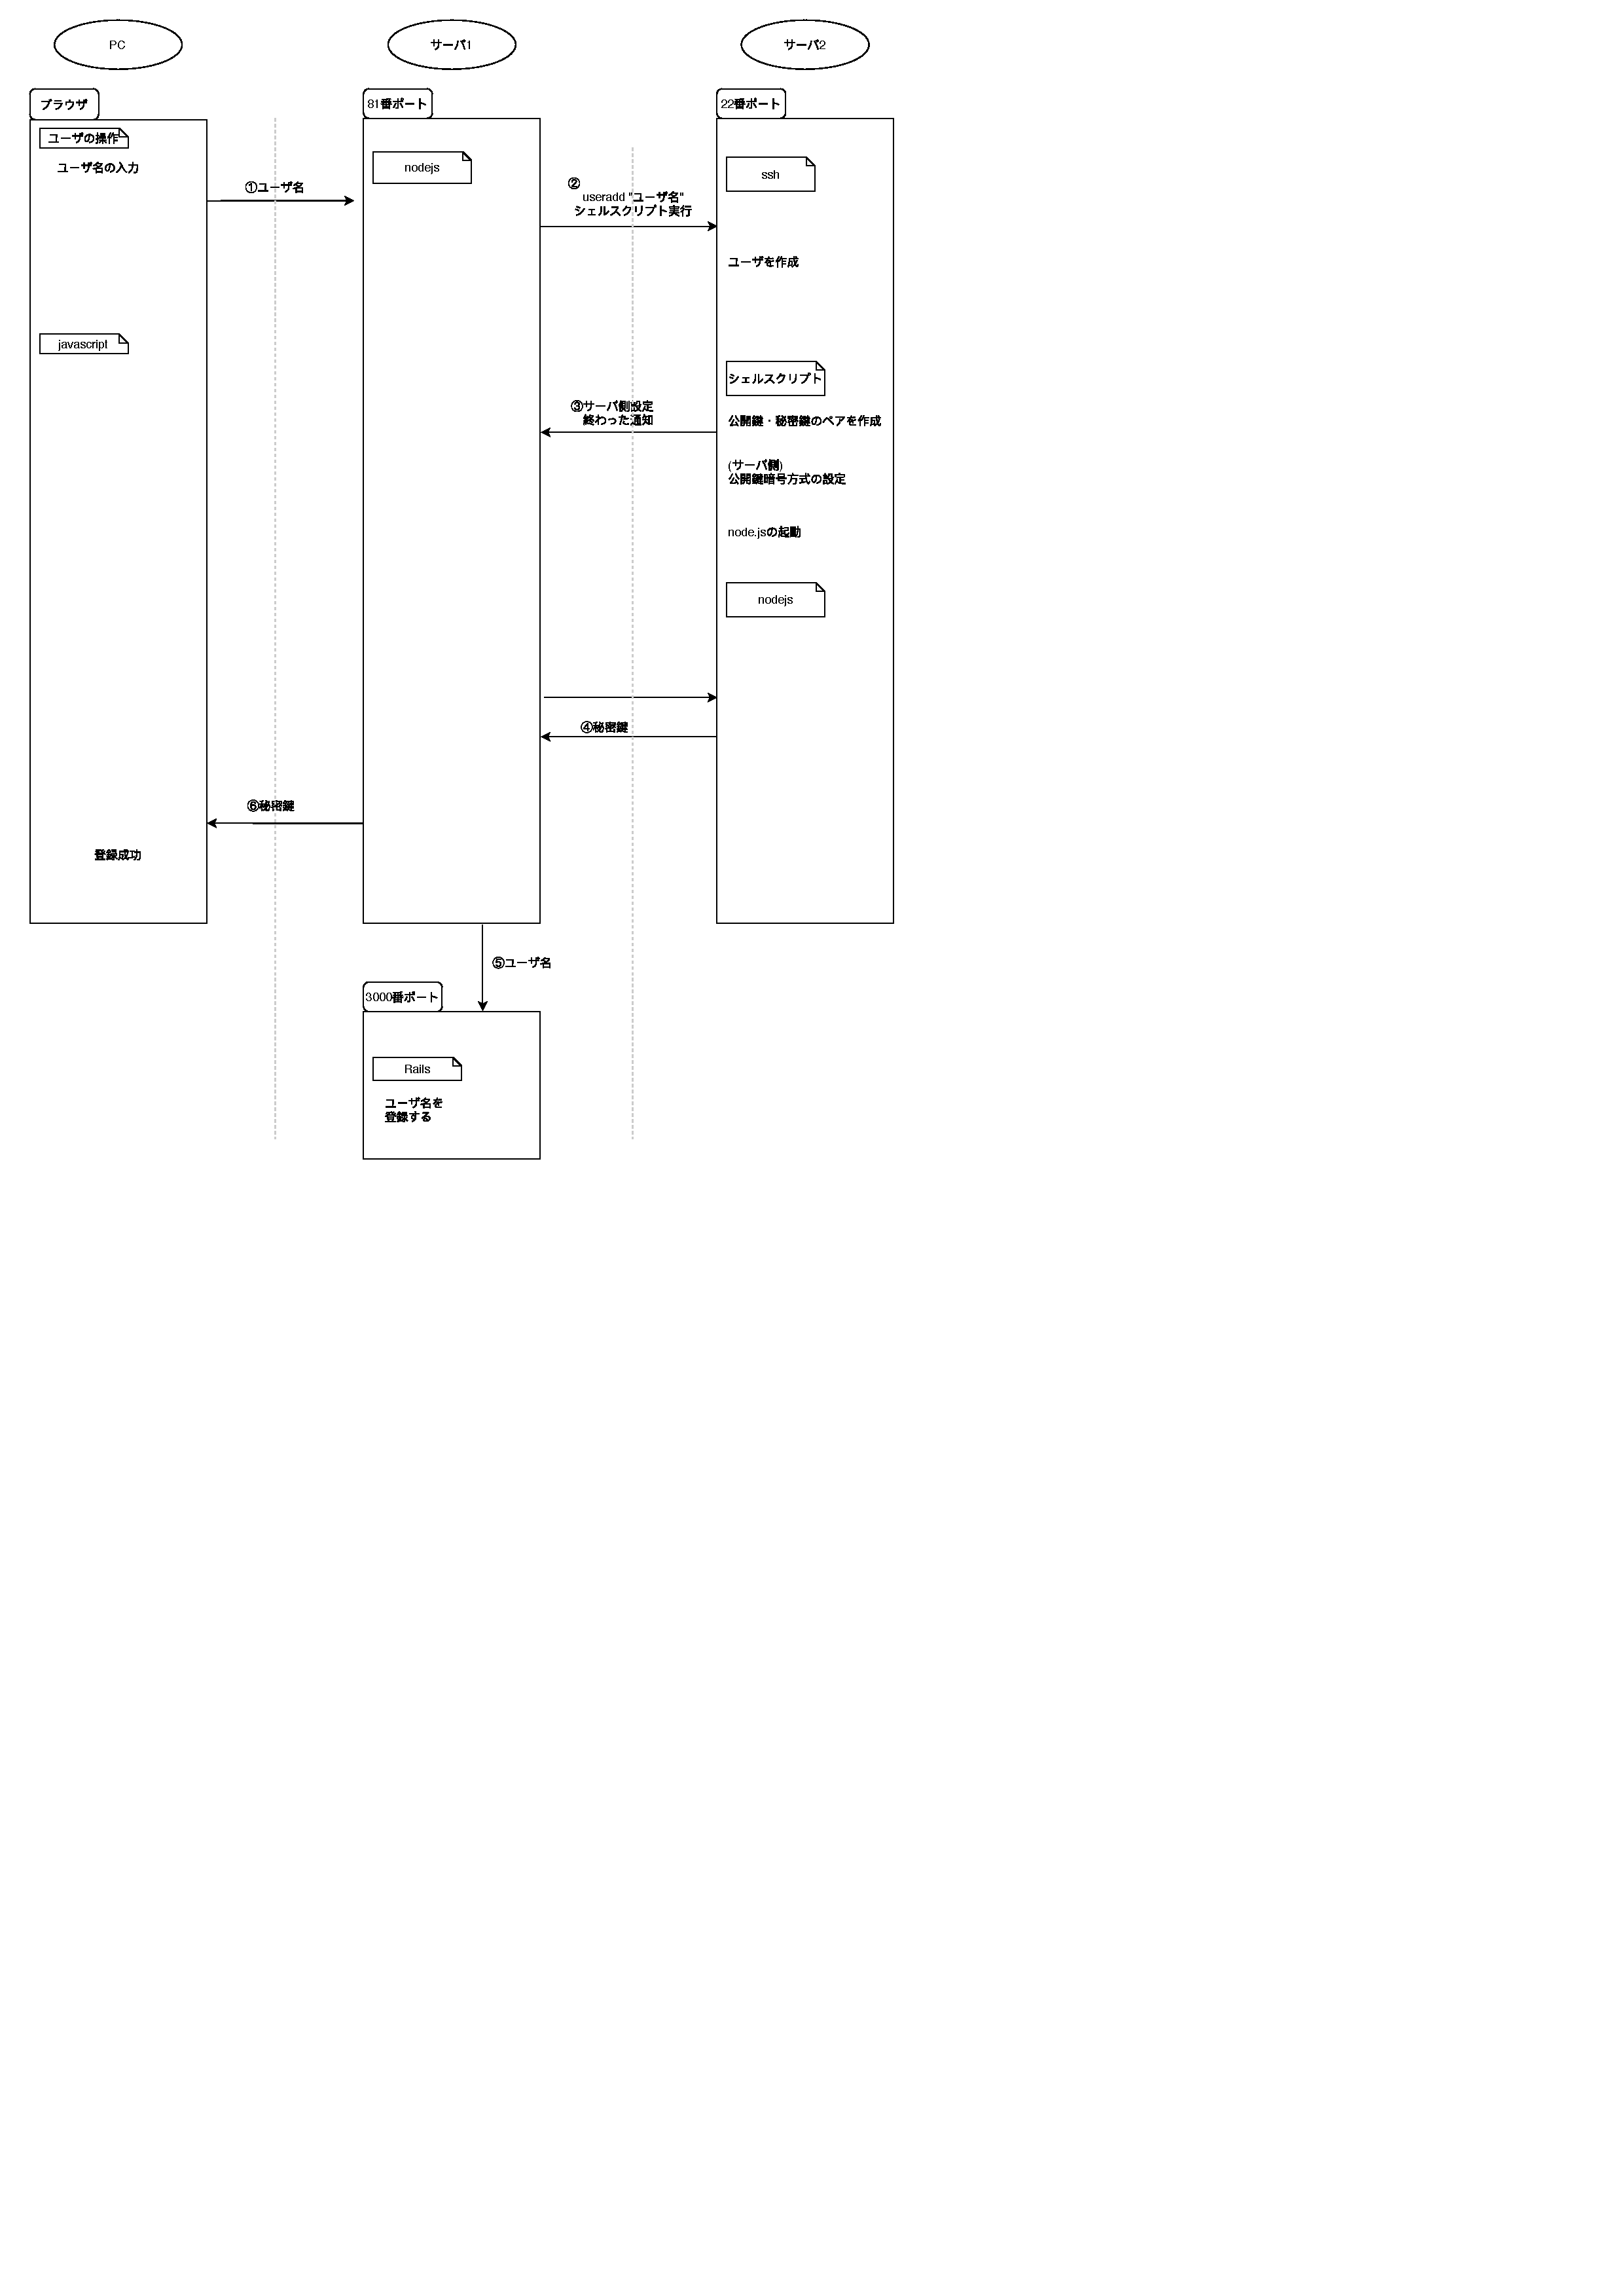
\includegraphics[width=13cm]{fig/chapter3/registration/key_register.pdf}
            \caption{鍵方式登録}
            \label{registration}
        \end{figure}
        %gitlubURL載せる?
    \subsection{認証}
        ここでは公開鍵暗号暗号方式による SSH を用いた認証から,WEBサービスの認証につなげる実装について記述する.
        以下の図\ref{certification}は実証の処理を記述した図である.
        %図を乗っける.
        \begin{figure}[H]
            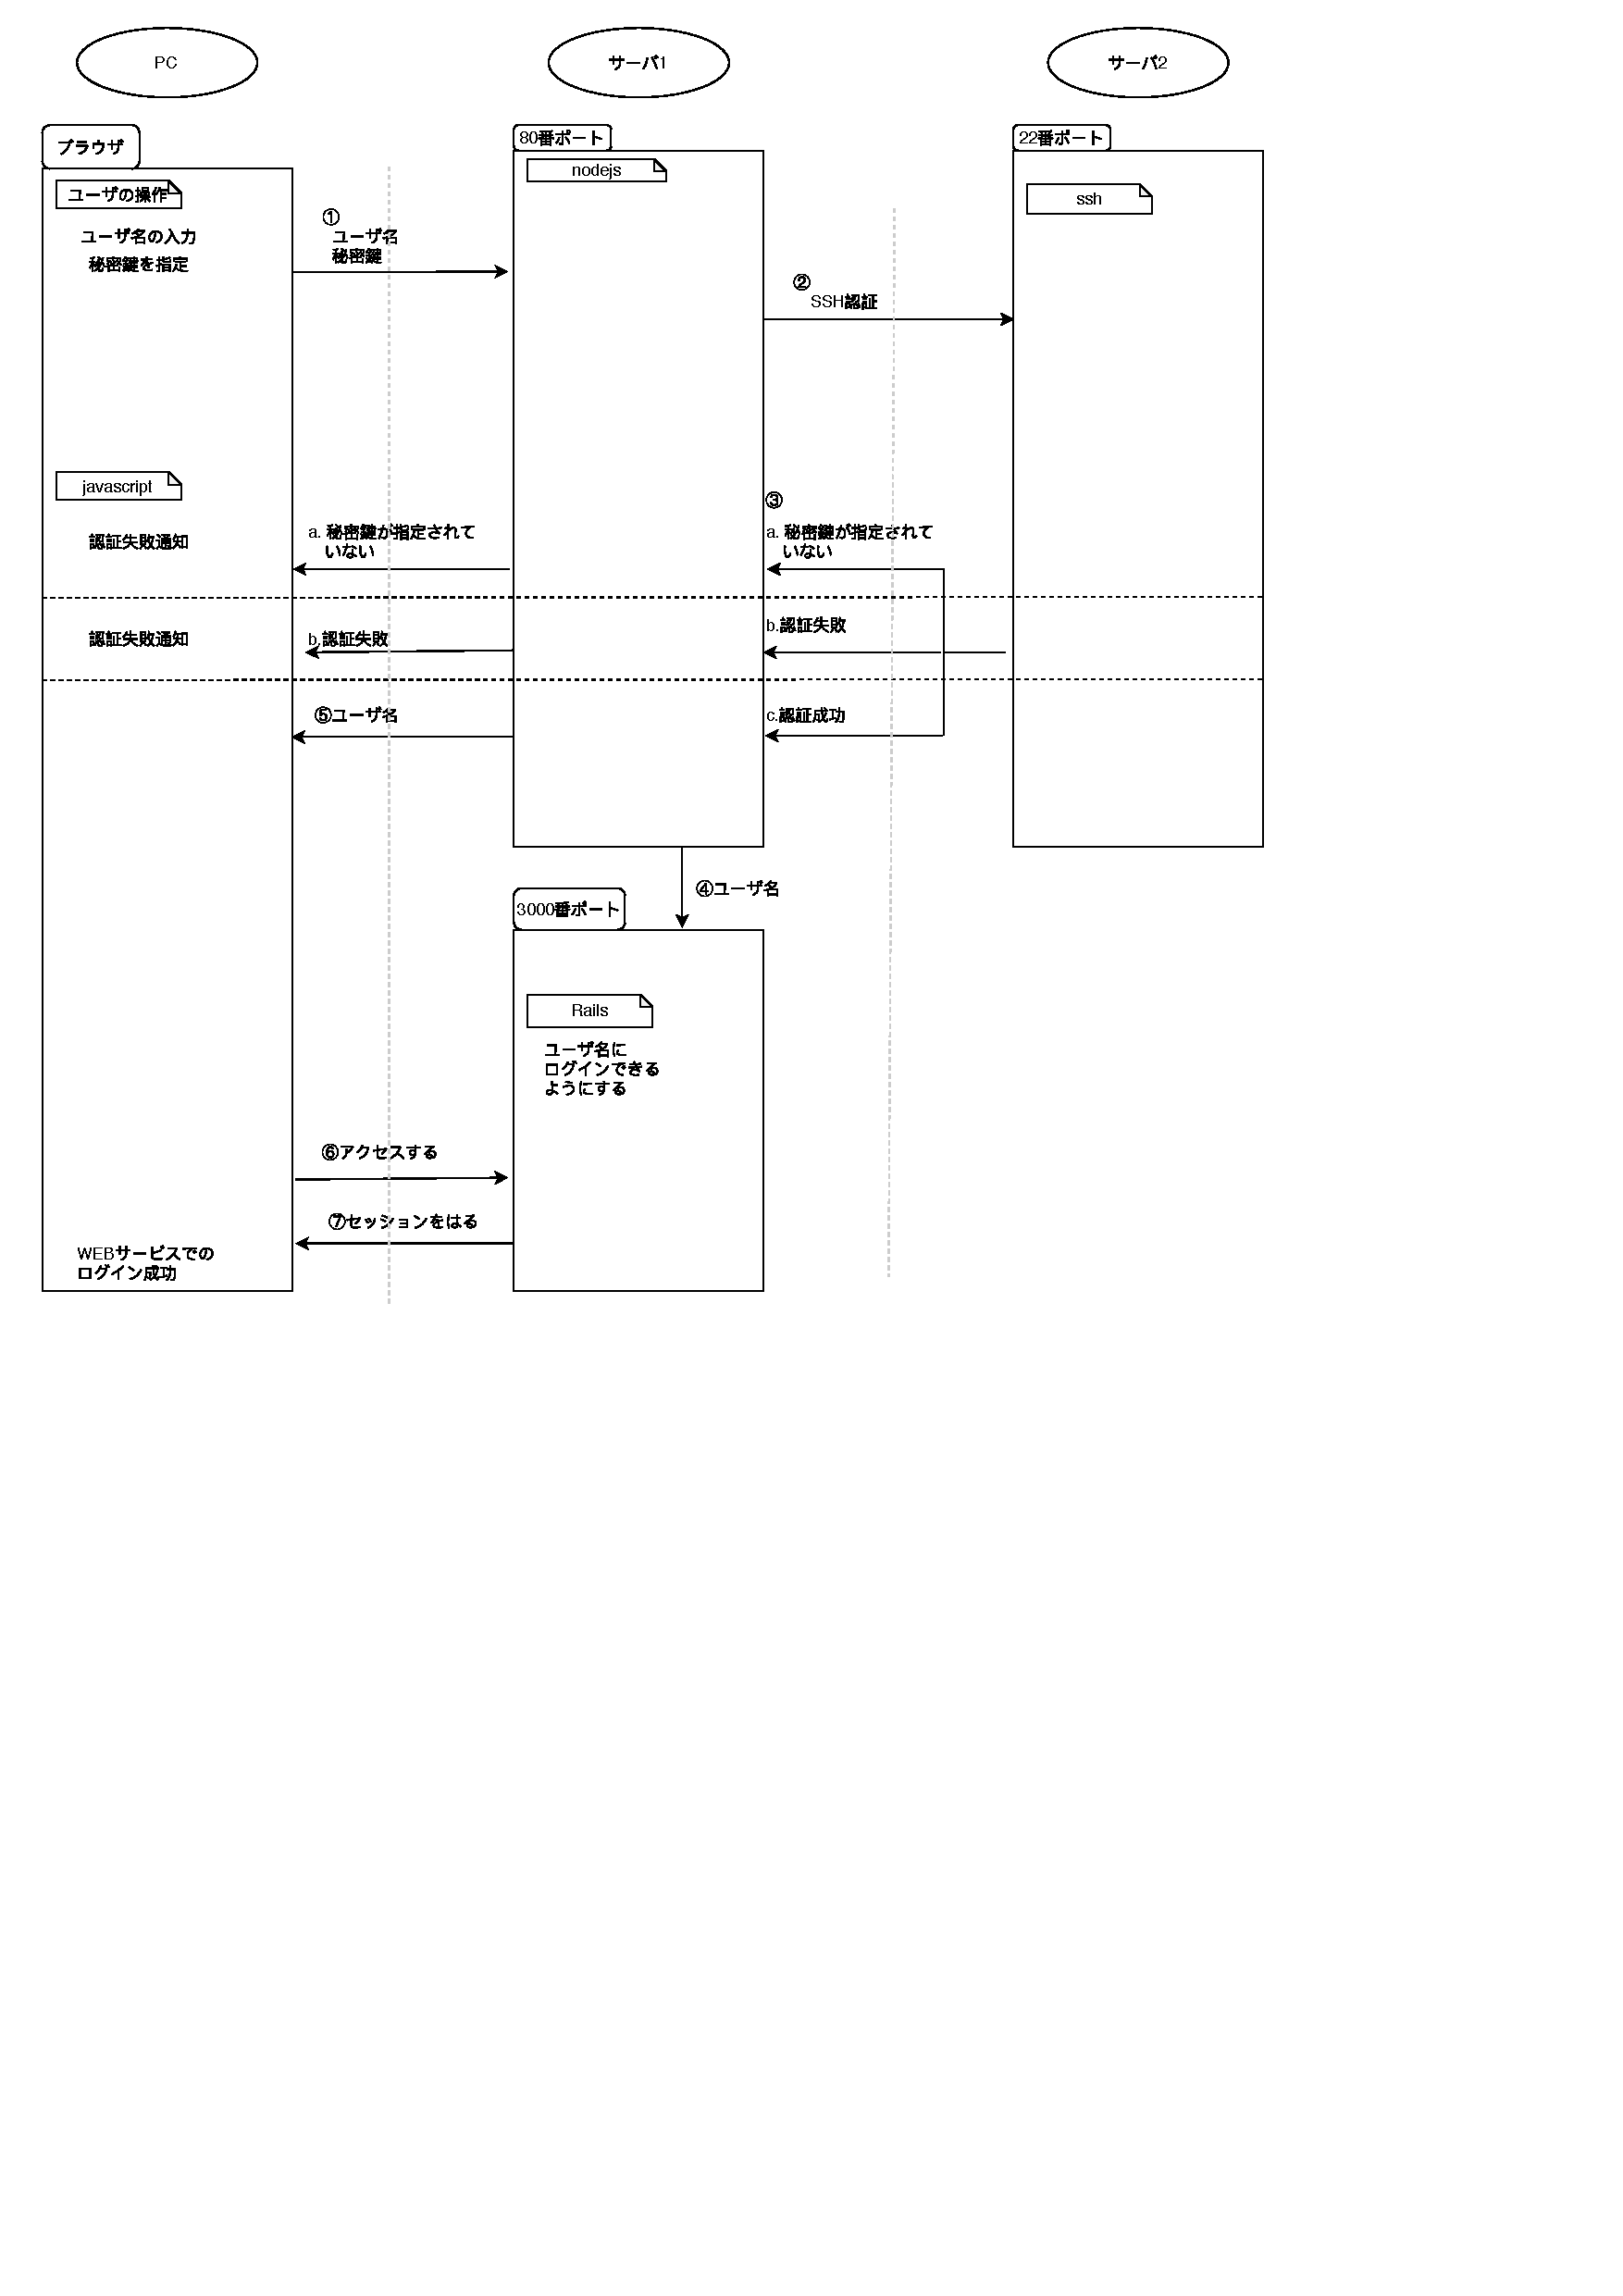
\includegraphics[width=13cm]{fig/chapter3/certification/key_certify.pdf}
            \caption{鍵方式認証1}
            \label{certification}
        \end{figure}


        %説明する.(図を用いながら)
        %gitlubURL載せる?

\section{パスワード方式の登録・認証の実装}
ここでは,
パスワード方式の登録・認証は検証で比較対象として用いる.
Railsチュートリアルのサイト\cite{Rails tutorial}を参考に最低限の作成をした.
参考にした,章・節・項を以下に列挙する.
\begin{itemize}
    \item 第6章 ユーザモデルの作成
    \begin{itemize}
        \item 6.1 Userモデル
        \begin{itemize}
            \item 6.1.1
            \item 6.1.2
        \end{itemize}
    \end{itemize}

    \item 第7章 ユーザ登録
    \begin{itemize}
        \item 7.1 ユーザを表示する
        \begin{itemize}
            \item 7.1.2
        \end{itemize}
        \item 7.2 ユーザ登録フォーム
        \begin{itemize}
            \item 7.2.1
            \item 7.2.2
        \end{itemize}
        \item 7.3 ユーザ登録失敗
        \begin{itemize}
            \item 7.3.1
            \item 7.3.2
        \end{itemize}
        \item 7.4ユーザ登録成功
        \begin{itemize}
            \item 7.4.1
            \item 7.4.2
        \end{itemize}
    \end{itemize}

    \item 第8章 ログイン,ログアウト
    \begin{itemize}
        \item 8.1 セッション
        \begin{itemize}
            \item 8.1.1
            \item 8.1.2
            \item 8.1.3
            \item 8.1.4
        \end{itemize}
        \item 8.2 ログイン
        \begin{itemize}
            \item 8.2.1
            \item 8.2.2
            \item 8.2.3
            \item 8.2.5
        \end{itemize}
    \end{itemize}

    \item 第9章 発展的なログイン機構
    \begin{itemize}
        \item 9.2 認可
        \begin{itemize}
            \item 9.2.1
            \item 9.2.2
        \end{itemize}

    \end{itemize}


\end{itemize}

    \begin{itemize}
        \item
    \end{itemize}


%gitlubのURL載せる???

\section{ボツ案}
\subsection{ログイン状態のセッション橋渡し}
\noindent 実装したいこと\\
公開鍵暗号方式によるssh認証を成功した際に,WEBサービスでログイン状態になる.
ここでいう,ログイン状態は,セッションを用いて,ステートフルな通信をする(HTTP通信はステートレスな通信).
\\\\
\noindent 実装するための手段案\\
ログイン状態のセッション情報を橋渡しすることにより,実現しようと考案した。以下の図\ref{botu1-1}を用いながら説明する。

\begin{figure}[h]
    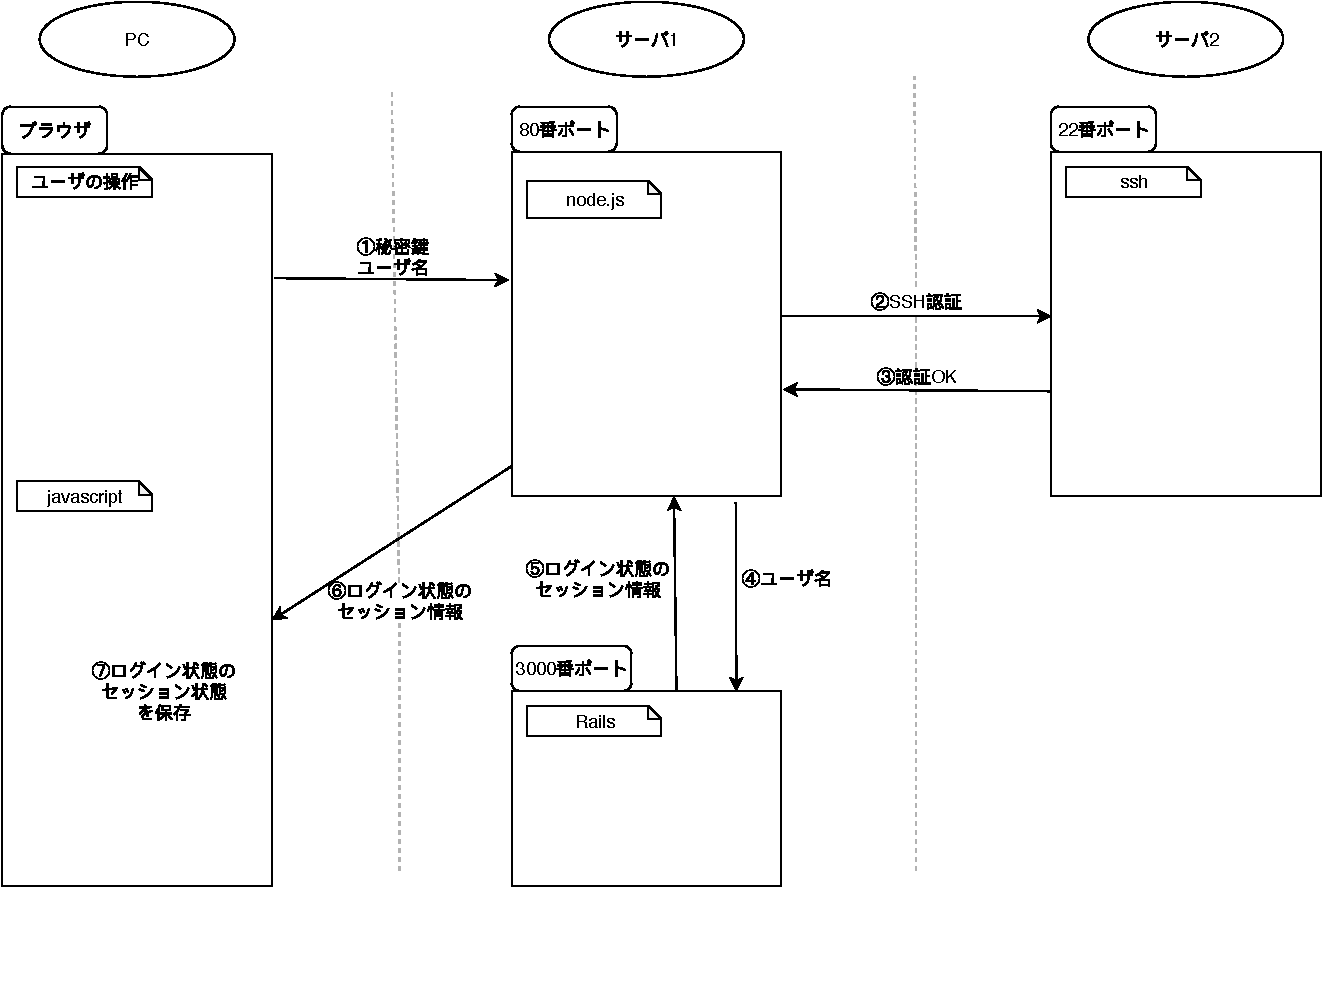
\includegraphics[width=13cm]{fig/chapter3/botu1-1.pdf}
    \caption{ログイン状態のセッション橋渡し案} 
    \label{botu1-1}
\end{figure}

%図を用いて(①とか)説明する
\noindent 図\ref{botu1-1}の\textcircled{\scriptsize 1} 〜 \textcircled{\scriptsize 3}では,エンドユーザはブラウザを用いて,公開鍵暗号方式によるsshをしている。
図\ref{botu1-1}の\textcircled{\scriptsize 4}では,HTTPリクエストのPOSTをしている。
図\ref{botu1-1}の\textcircled{\scriptsize 5}では,HTTPレスポンスが来て,そのヘッダ情報に「セッション情報をCookieに保存する」という情報が付与されている(のちのち,アクセス制限で,localhostからしかアクセスできないようにする).
図\ref{botu1-1}の\textcircled{\scriptsize 6}では,図\ref{botu1-1}の\textcircled{\scriptsize 5}の情報を,ブラウザのjavascript側にsocket通信で渡す.
最後に,図\ref{botu1-1}の\textcircled{\scriptsize 7}で,ログイン状態のセッション情報をCookieに保存する.
\\\\
\noindent ブラウザを用いての検証\\
ログイン中のセッション情報を,ブラウザのCookieに保存することで,ログインすることが可能かを検証する。\\
検証環境\\
 \quad 機器\\
  \qquad MacBook Pro (Retina, 13-inch, Early 2015)\\
  \qquad macOS High Sierra(バージョン10.13.6)\\
 \quad サーバ側\\
 \qquad Ruby on Rails(6.0.2.1)\\
 \qquad localhost:3000\\
 \quad ユーザ側\\
 \qquad 2っのブラウザ\\
 \qquad \quad Google Chrome\\
 \qquad \quad Google Chrome Canary\\
Cromeの開発環境(デベロッパーツール)を用いて以下の検証を行った。\\
まず,ログインした際の動きとして,HTTPレスポンスのヘッダ情報に,set-cookieがある.Cromeのデベロッパーツールでは,以下の図\ref{login-1}と表示される.\\
 \begin{figure}[h]
    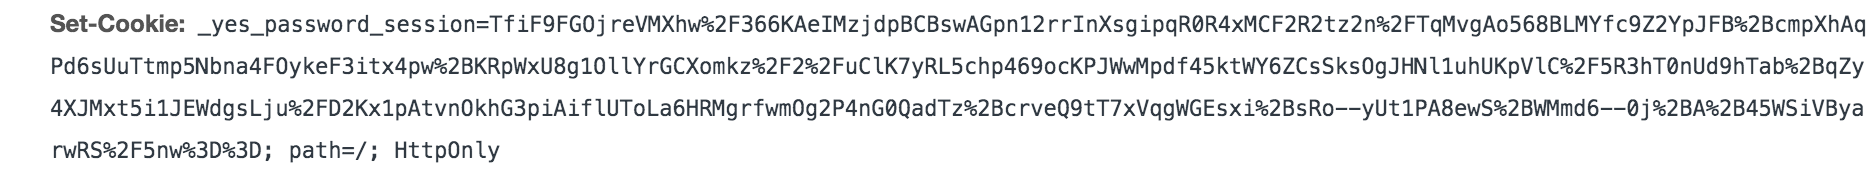
\includegraphics[width=13cm]{fig/chapter3/login-1.png}
    \caption{ログイン成功した際の,HTTPレスポンスの抜粋} 
    \label{login-1}
\end{figure}

\noindent 次に,図\ref{login-1}のHTTPレスポンスを元に,ブラウザのCookieにセッション情報を保存する。
Cromeのデベロッパーツールでは,以下の図\ref{login-2}と表示される.\\
\begin{figure}[h]
    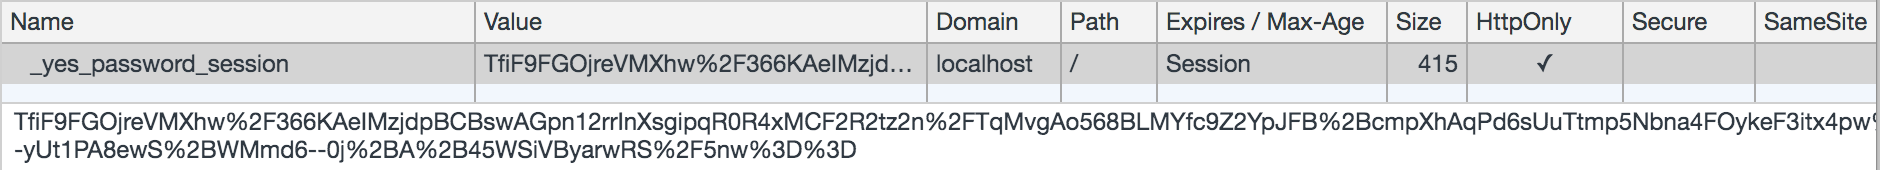
\includegraphics[width=13cm]{fig/chapter3/login-2.png}
    \caption{ブラウザのCookieのセッション情報}
    \label{login-2}
\end{figure}
上記の\ref{login-1},\ref{login-2}は,HTTPレスポンスのヘッダ情報で,ブラウザのCookieに値を保存している.その後,HTTPリクエストで,Cookie情報を付与\cite{cookie1}することにより,ステートレスなプロトコルであるHTTP上で,状態管理ができる\cite{cookie2}(ログイン状態の維持).
\\
現状で以下の図\ref{login_compare-1}のように,ログインしているブラウザ,ログインしていないブラウザがある.\\
\begin{figure}[h]
    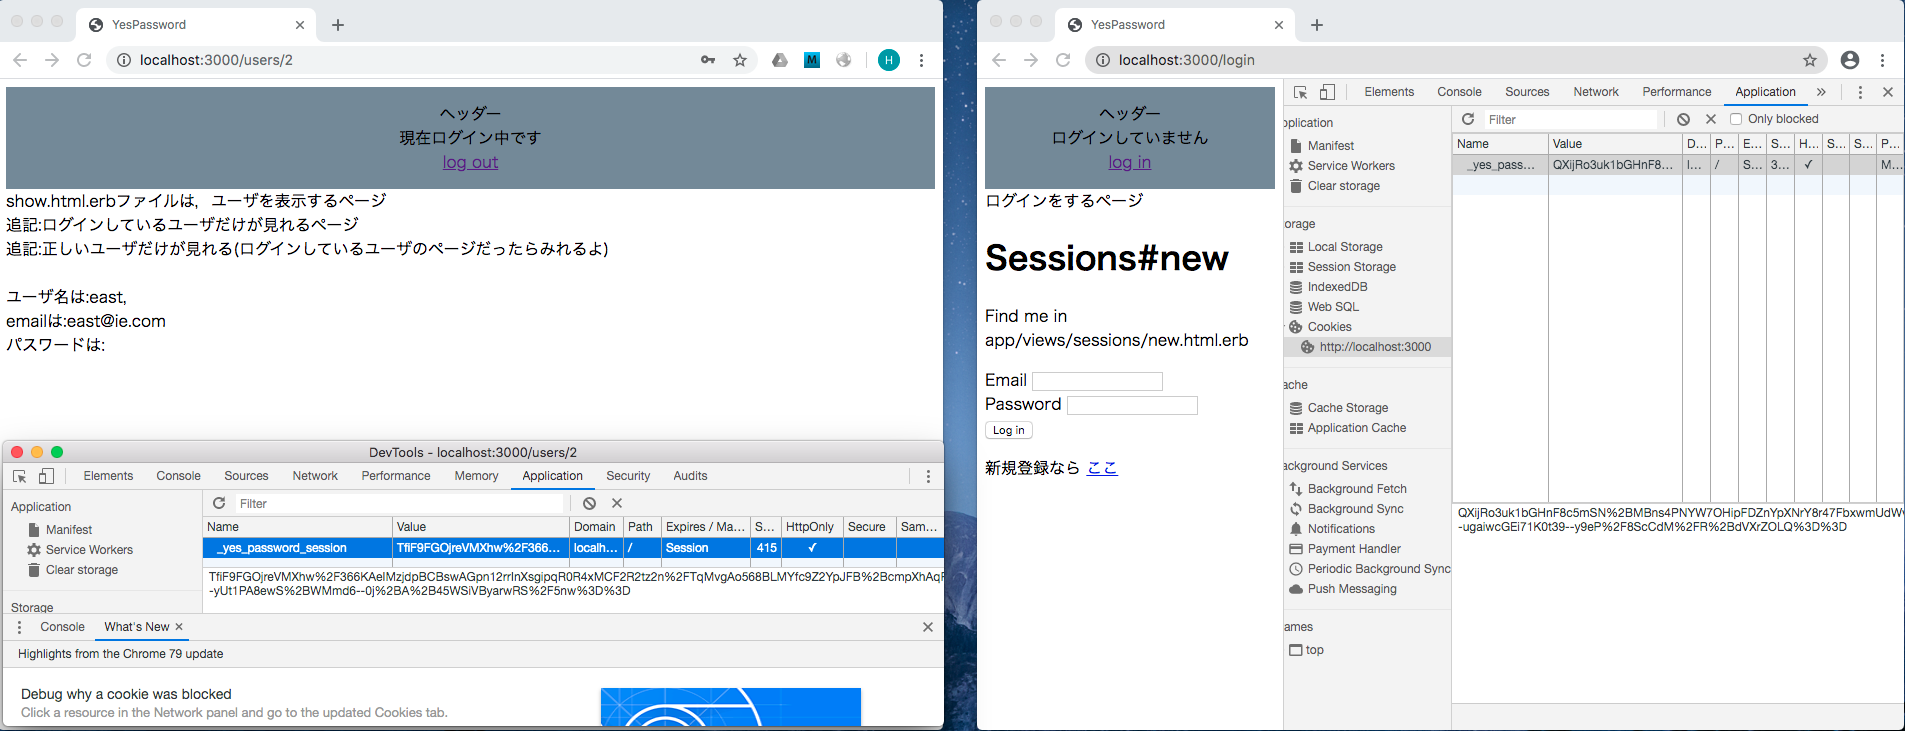
\includegraphics[width=13cm]{fig/chapter3/login_compare-1.png}
    \caption{2っのブラウザ(ログイン状態,ログインしていない状態)} 
    \label{login_compare-1}
\end{figure}
\\
上記の図\ref{login_compare-1}の状態から次の操作を行う.デベロッパーツールを用いて,ログインしているブラウザから,ログインしていないブラウザに,Cookie情報の,コピーアンドペーストを行い.リロードする.
その際の,状態が以下の図\ref{login_compare-2}になり,ログイン状態のセッションを橋渡し(Cookieに保存)することにより,ログインすることができることがわかる.\\
\begin{figure}[h]
    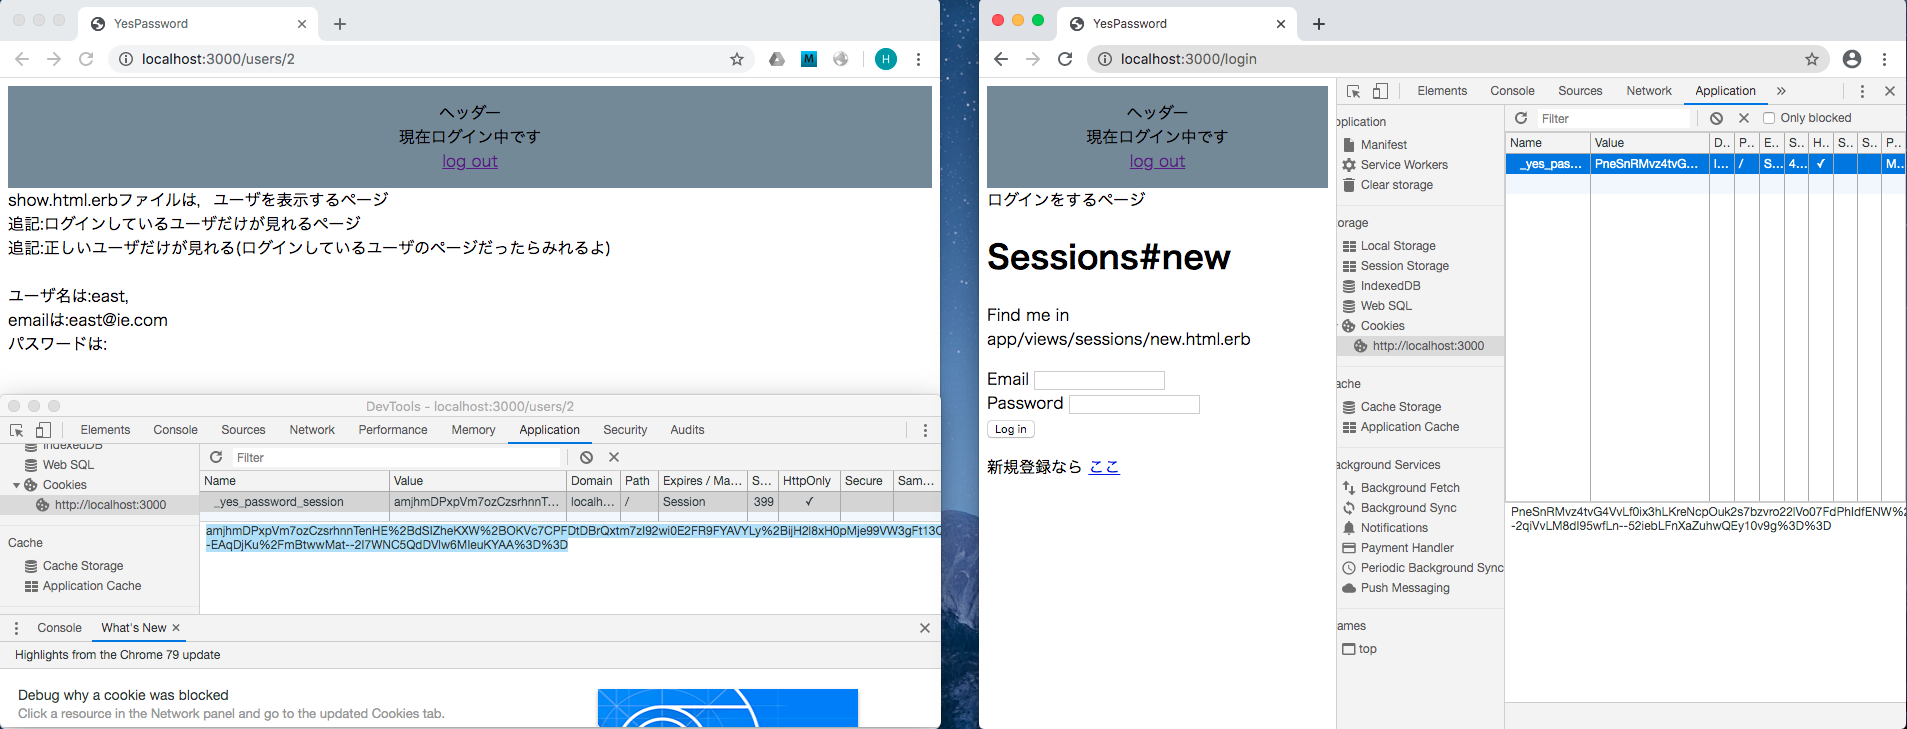
\includegraphics[width=13cm]{fig/chapter3/login_compare-2.png}
    \caption{2っのブラウザ(ログイン状態,ログイン状態)} 
    \label{login_compare-2}
\end{figure}
\\
図\ref{login_compare-2}の補足.\\
HTTPリクエストをする際に,新しいCookie情報が付与されることが確認できた.そのことにより,ログイン中の2っのブラウザが別のセッションになっている.
\\\\
\noindent 実際に実装\\
実際に実装を進めて,図\ref{botu1-1}の\textcircled{\scriptsize 1} 〜 \textcircled{\scriptsize 6}までできた.しかしながら,図\ref{botu1-1}の\textcircled{\scriptsize 7}ができなかった.その理由を以下の図\ref{botu1-2.pdf}を元に説明する.
\begin{figure}[h]
    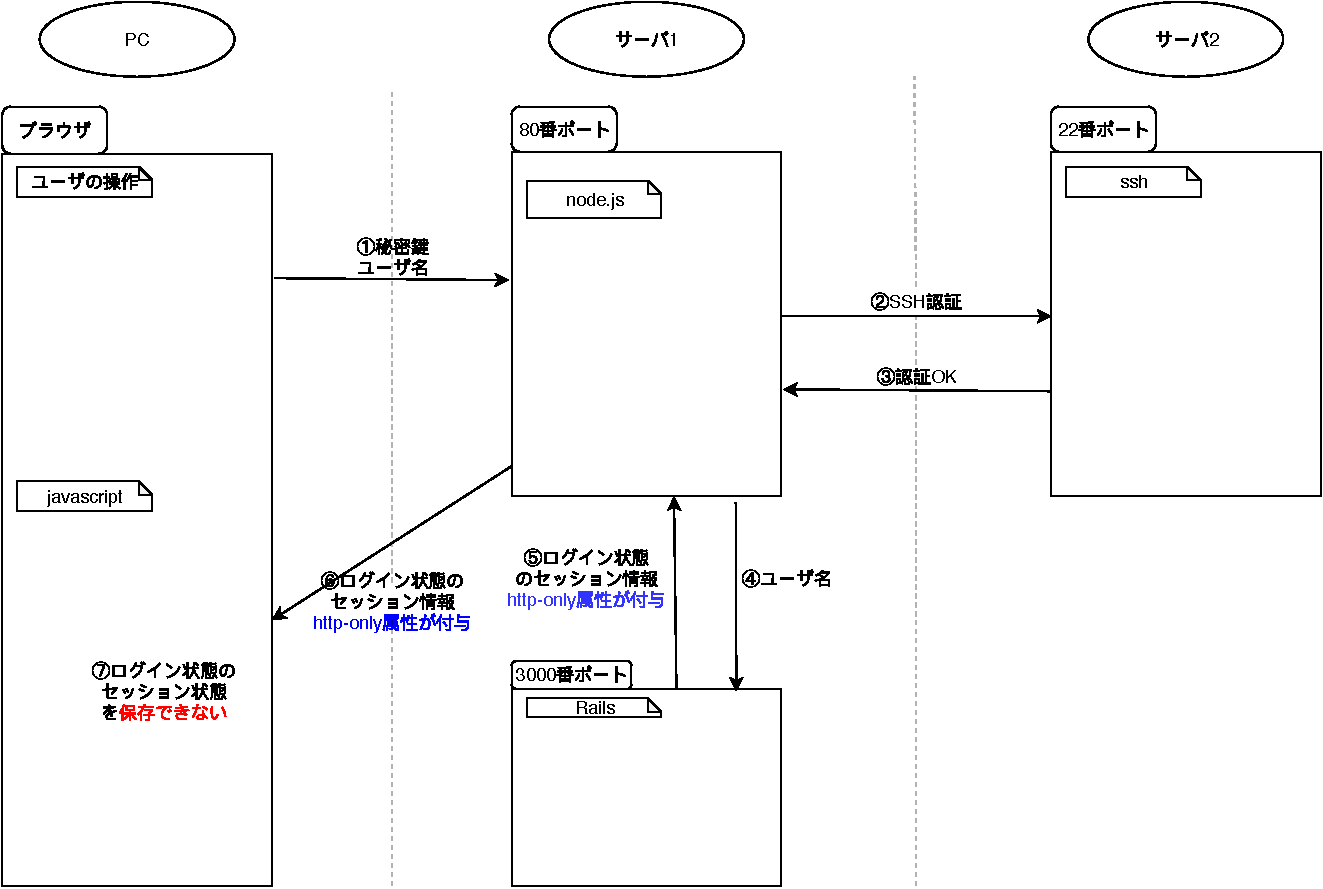
\includegraphics[width=13cm]{fig/chapter3/botu1-2.pdf}
    \caption{ログイン状態のセッション橋渡し案がボツになった} 
    \label{botu1-2.pdf}
\end{figure}
\\
図\ref{botu1-2.pdf}の\textcircled{\scriptsize 5} で,railsではセッションを発行する際に,http-only属性を付与している\cite{cookie-httponly-default}.そのことは,ログイン時のHTTPレスポンスである図\ref{login-1}でも現れている.
http-only属性がついたCookieは,javascriptで扱うことができなくなり,セッションハイジャックの対策を行っている\cite{cookie-httponly-security}.
そのため,図\ref{botu1-2.pdf}の\textcircled{\scriptsize 7}のように,セッション状態を保存することができなかったため,「ログイン状態のセッション橋渡し」の案はボツになった.
%
%
%図を用いながら,できない説明。
%  ( 図で,考案のどこまでできたかを示そうマル6までできたが,⑦でできなかった)
%そのためこの案はボツになった
